% *********************************************************************
% © 2021 Jeremy Sylvestre
%
% Permission is granted to copy, distribute and/or modify this document
% under the terms of the GNU Free Documentation License, Version 1.3 or
% any later version published by the Free Software Foundation; with no
% Invariant Sections, no Front-Cover Texts, and no Back-Cover Texts. A
% copy of the license is included in the appendix entitled “GNU Free
% Documentation License” that appears in the output document of this
% PreTeXt source code. All trademarks™ are the registered® marks of
% their respective owners.
%
% *********************************************************************

\newcommand*{\xmin}{-0.5}
\newcommand*{\xmax}{6}
\newcommand*{\ymin}{-11.5}
\newcommand*{\ymax}{7.5}

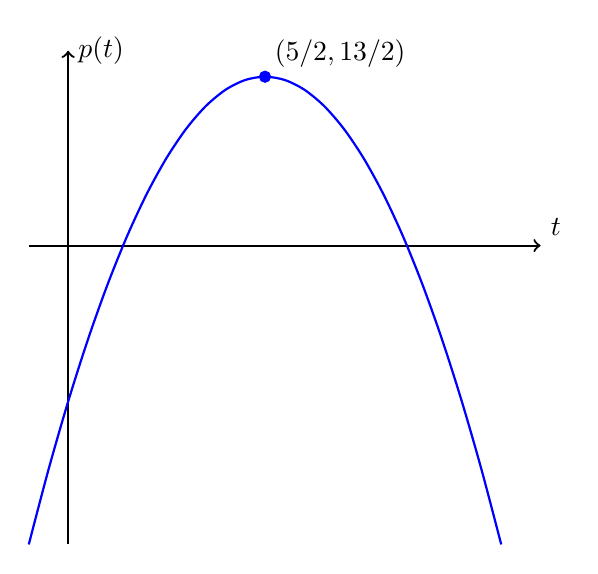
\begin{tikzpicture}
[
	closedpt/.style={circle,draw,fill,inner sep=0pt,minimum size=4pt},
	openpt/.style={circle,draw,inner sep=0pt,minimum size=4pt},
	yscale=0.33
]

	% axes
	\draw[->,thick] (\xmin,0) -- (\xmax,0) node[above right] {$t$};
	\draw[->,thick] (0,\ymin) -- (0,\ymax) node[right] {$p(t)$};

	\draw[blue,thick,domain=-0.5:5.5,smooth] plot (\x,{- 2 * \x * \x + 10 * \x - 6});

	\node[blue,closedpt] at (2.5,6.5) {};
	\node[above right] at (2.5,6.5) {$(5/2,13/2)$};

\end{tikzpicture}
